\documentclass[emulatestandardclasses]{scrartcl}
\usepackage{graphicx}
\usepackage{color}
\usepackage[ngerman]{babel}
\usepackage{hyperref}
\usepackage{fullpage}
\usepackage{calc} 
\usepackage{enumitem}
\usepackage{titlesec}
\newcommand{\todo}[1]{\textcolor{red}{TODO: #1}\PackageWarning{TODO:}{#1!}}
\date{\vspace{-3ex}}
\begin{document}

\title{
	\includegraphics*[width=0.75\textwidth]{ErstesSem/images/hu_logo.png}\\
	\vspace{24pt}
	Merleau-Ponty: Ph"anomenologie der Wahrnehmung}
\subtitle{Proseminar SS 17\\
          Matthias Schlo"sberger\\
          Philosophisches Institut I \\ 
          Humboldt Universit"at zu Berlin}
\author{Lennard Wolf\\
        \small{\href{mailto:lennard.wolf@student.hu-berlin.de}{lennard.wolf@student.hu-berlin.de}}}
\maketitle
\begin{abstract}

Anhand eingehender Lekt"ure von Maurice Merleau-Pontys "`Ph"anomenologie der Wahrnehmung"' soll der ph"anomenologische Begriff des „Leibes“ rekonstruiert werden. Dabei geht es zun"achst um das Verh"altnis des eigenen Leibes zur Umwelt, im weiteren Verlauf dann um das Verh"altnis zu den Anderen. Der ph"anomenologische Begriff des Leibes, so die These, bietet eine Möglichkeit, die Extreme des Empirismus (= naturwissenschaftliche Verdinglichung des Leibes als K"orper) und des Intellektualismus (= idealistische Ausklammerung des Leibes) zu unterlaufen. Besondere Aufmerksamkeit gilt den Ausführungen zu Gestaltpsychologie und Entwicklungspsychologie. Das Proseminar richtet sich insbesondere an Studienanf"anger.

\end{abstract}
\newpage

\tableofcontents
\listoffigures
\newpage


\section{Einf"uhrung\\(20.04.17)}

\subsection{Einf"uhrung}
\subsubsection{Was ist Ph"anomenologie?}

\begin{itemize}
  \item Bewusstseinsforschung: Husserl sp"ater: Transzendentale Ph"anomenologie / R"uckkehr zum Objekt
  \item Husserl: \emph{Logische Untersuchen} (1900 - 1901) Grundschrift aber viele wichtige Thesen fehlen noch
  \item "`Psychologismus"': Alles was man wahrnimmt/denkt ist abh"angig von der psycho-physischen Organisisation des Gehirn | Wird von Husserl kritisiert durch die Untersuchung universaler Strukturen
  \item Bewusstsein hat Aktcharakter, muss dies aber nicht haben
  \item Bewusstsein hat \emph{Bezogenheit} auf $X$ - auch: Intentional gerichtet (aber sprachlich unsauber, denn: Bewusstsein ist immer intentional und damit gerichtet $\rightarrow$ Doppelung) -- Intention: Verbindung zwischen Subjekt und Objekt
  \item Besonderes an dem Modell: 
  \item R"uckf"uhrung: Wie baut sich Erkenntnis auf? $\rightarrow$ Basale Kategorien/Einfachste Erfahrung? $\rightarrow$ Wie kommen wir zu einer Ontologie? Wie rechtfertigen wir diese?
  \item Vorgehen: Was sind die basalen Kategorien? $\rightarrow$ Wie begr"unden wir unsere Kategorie? $\rightarrow$ ?
  \item Ph"anemonologische Erkenntnistheorie: \emph{Sinnauslegung}, nicht "`Sinngebung"'
  \item Warum macht es Sinn zu fragen, wie wir eine Ontologie aufbauen?
  \item Entwicklungspsychologie \& Erkenntnistheorie: Parallel oder nacheinander?
  \item Hegels Kritik an Erkenntnistheorie: "`Wer theretisch verstanden hat, wie das Schwimmen funktioniert, der kann noch nicht schwimmen. Wer schwimmen kann, muss keine Theorie des Schwimmens haben."'
  \item Die beste Theorie ist der Akt selber? Das beste Modell ist das Ding selber?
  \item Was machen wir wenn wir die Erfahrung des anderen machen?
  \item Ph"anemonelogische Reduktion: Rekostruktion der Wahrnehmungsleistung durch Ausklammerung aller schon bekannten Erfahrung
  \item Erste Unterscheidung: Ich $\longleftrightarrow$ Welt
  \item \emph{Leib}: 
  \item Differenz Leib und K"orper? Ich sehe den Leib des anderen -- fundamental anders als zu sagen ich sehe den K"orper eines anderen
  \item Urspr"unglich nehmen wir den Leib war, der K"orper ist nur eine abstrakte Wahrnehmungsleistung (Ich muss zuerst den Leib wahrnehmen, bevor ich den K"orper wahrnehmen kann)
  \item Zu n"achster Sitzung: Vorwort \& Einleitung 
  
\end{itemize}

\section{Vorwort\\(27.04.17)}

\subsection{Lekt"urenotizen}

\begin{itemize}
  \item "`I cannot conceive myself as nothing but a bit of the world, a mere object of biological, psychological or sociological investigation"'
  \item But the relations between subject and world are not strictly bilateral
  \item I cannot put perception into the same category as the syntheses represented by judgements, acts or predications. 
  \item Perception is presupposed by all acts
  \item there is no inner man, man is in the world, and only in the world does he know himself
\end{itemize}

\subsection{Kontext}

\begin{itemize}
  \item 1945 ver"offentlicht, schwierige Phase der phen. Bewegung (Husserl Tod 1930)
  \item Erste Generation in Vergessenheit geraten, besonders Max Scheeler
  \item Projekt hat sich auf Existenzphilosophie Heideggers zubewegt
  \item Merleau-Ponty: Zur"uck zu Husserl, obwohl in Misskredit geraten
  \item Ph"anemonologie lebt von "`Trennung"' (?)
  \item Transzendentale Subjektivit"at: Es soll gezeigt werden, dass alle das Ding gleich erleben (?) (das Dreieck ist f"ur alle Egos das gleich) $\rightarrow$ Es wird nicht relativ nur weil es von einem Subjekt wahrgenommen wird
  \item "`Zu den Sachen selbst"' Dinge werden \emph{konstituiert}, nicht konstruiert
  \item Husserl am Ende des Lebens: \emph{Reduktion} als neue Operation ("`Die Idee der Ph"anomenologie"', 1913)
  \item "`Ph"anomenologische Bewegung"' beginnt wenn Farber auf dem Fahrrad zu Husserl f"ahrt und die verbreitet die "`Lehre"' zwischen M"unchen und G"ottingen (nah an den logischen Untersuchungen), emp"ort bei der transzendentale Wendung kommt ("`R"uckschritt"'?)
  \item Unterscheidung "`Idealistische Ph"anomenologie"' und "`Realistische Ph"anomenologie"' (letztere macht transzendentale Wendung Husserls nicht mit)
  \item Fragestellung verschiebt bei diesem Disput $\rightarrow$ Merleau-Ponty: "`Wir m"ussen auf Husserl zur"uckgehen. Die Differenzen in den Ph"anomenologien sind nicht so gro"s, wir kommen nicht ohne die Fundierung Husserls aus."'
\end{itemize}

\subsection{Vorwort}

\begin{itemize}
  \item Da-Sein So-Sein
  \item Wie anthropologisch ist die Theorie? Sp"ater
  \item "`For if I am able to talk about ‘dreams’ and ‘reality’, to bother my head about the distinction between imaginary and real, and cast doubt upon the ‘real’, it is because this distinction is already made by me before any analysis; it is because I have an experience of the real as of the imaginary"' $\rightarrow$ Unterscheidung wirklich/gedacht | WEIL: Wir k"onnen nicht \emph{logisch schlie"sen} dass wir in der Wirklichkeit sind (weil wir daf"ur schon mit ihr vertraut sein m"ussen), also m"ussen wir die Wirklichkeit daf"ur einfach \emph{erleben}, wir nehmen es also grunds"atzlich an
  \item Warum ist R"uckf"uhrung von .... bezeichnet als Transzendentalphilosophie?
  \item "`For a long time, and even in recent texts, the reduction is presented as the return to a transcendental consciousness before which the world is spread out and completely transparent, quickened through and through by a series of apperceptions which it is the philosopher’s task to reconstitute on the basis of their outcome"'
  \item If we were absolute mind, the reduction would present no problem. But since, on the contrary, we are in the world, since indeed our reflections are carried out in the temporal flux on to which we are trying to seize (since they sich einströmen, as Husserl says), there is no thought which embraces all our thought.
  \item Zur n"achsten Sitzung: Was bedeutet \emph{Schauen} (nicht nur optisch) und: Wie k"onnte eine phen. Diskussion aussehen im Gegensatz zu einer philosophischen? | Lesen: 
\end{itemize}


\begin{description}[leftmargin=!,labelwidth=\widthof{\bfseries Transzendentalphilosophie bei Kant}]
  \item[Ph"anomenologie] Wesensforschung, versetzt alles Wesen zur"uck in die Existenz, stellt die Frage "`Was ist Wirklicheit/Wie wird sie wahrgenommen?"', ist Transzendentalphilosophie
  \item[Existenz] 
  \item[Transzendentalphilosophie bei Kant] 
   \item[Transzendentalphilosophie bei MP] 
  \item[Nat"urlich] In jedem normalen unreflektierten Bewusstseinsleben sind wir in der nat"urlichen Einstellung. "`Die Welt ist einfach da."' 
  \item[Eidetisch] Bildhaft, anschualich
  \item[Transzendentale Reduktion] Ziel: Frage nach wie wir von dem Ding an sich ausgehen k"onnen, auch wenn wir es nicht 
  \item[Eidetische Reduktion] Ziel: Regionale Ontologien | Ohne Urteilskraft wahrnehmen / nat"urliches Wahrnehmen
  \item[Ph"anomenologische Reduktion] Auf den Erfahrungsboden der Wahrnehmung zur"uckkehren, zur"uck zum Wesen der Dinge
  \item[Wesen] Wesen des Dreiecks ist von den existierenden Dreiecken unabh"angig, unabh"angig von der psycho-physischen Struktur
\end{description}


\section{Einleitung I\\(03.05.17)}

\subsection{Empfindung}

\begin{itemize}
  \item "`Die klassischen Vorurteile und R"uckgang auf die Ph"anomene"'
  \item Warum gerade mit der Erfahrung beginnen? Weil es m"oglicherweise Grundlage f"ur den Kontakt mit der Welt ist 
  \item Ist es notwendig sich mit den klassischen Antworten zu den Fragen der Ph"anomenologie? Ja! Durch den Vergleich zeigen wir wie wichtig Ph"anomenologie als Wissenschaft ist. Und damit die Begriffe die wir verwenden nicht unbekannterweise schon zu bedeutungsschwanger sind.
  \item Empfindungen sind durch die Sinne vermittelt -- Sinn loswerden?
  \item Wenn man kein Vokabular für die Farben hat, (wie) nimmt man sie wahr?
  \item Sinnbegriffe sind immer doppeldeutig
  \item Reine empfindung: Dass es etwas gibt, wie ein reines f"uhlen, das nicht irgendwie mit einem \emph{Auffassen} verkn"upft. M-P bestreitet dass es das gibt!
  \item Wahrnehmung: \emph{etwas} wahrnehmen
  \item Qualit"aten sind nie unmittelbar erlebt und jedes Bewusstsein ist Bewusstsein \emph{von etwas} ist
  \item Wenn ich mir einer Empfindung nicht bewusst bin, empfinde ich sie auch nicht.
  \item Bewertung von EMpfindungen ist vorsprachlich
  \item Auffassen: Vorsprachliche Sinngebung der Empfindung
  \item Bewusstsein fasst immer auf, Ohne Bewusstsein gibt es keine Empfindung $\rightarrow$ Es gibt keine reine Empfindung.
  \item Empfindung k"onnte die primitivste Form des Bewusstseins sein. 
  \item Objektive Wahrnehmung kann es nicht geben da die daf"ur gebrauchte Messlatte nur durch die subjektive Wahrnehmung entwickelt werden kann und damit schon
  \item Frei machen von "`realistischem Modell"' (freimachen von dem Ziel des Zugriffs auf Objektivit"at, wir nehmen die Welt war sie ist (?))
  \item Idealistische Wahrnehmung als Ziel? Oder Realistische? Scheinbar nicht ganz klar...
  \item Zur n"achsten Sitzung: II + III
\end{itemize}

\subsection{Nacharbeit}

\begin{itemize}
  \item Ist reine Empfindung also eine "`nicht bewusste"'?
  \item Bildet die Grundlage f"ur Bewusstsein weil durch sie etwas wahrgenommen werden kann?
  \item Empfindung ist die Urgrundlage des Bewusstseins, denn Wahrnehmen ist Bewusstsein (?)
\end{itemize}


\section{Einleitung II + III\\(10.05.17)}

\subsection{Lekt"urenotizen}


\textbf{\S 5.} Was ist der "`Sinn"' von Ausdr"ucken die Impressionen bezeichnen? Wo kommt der her? $\rightarrow$ Impressionen sind nicht nur punktuell, sondern auch komplex (wieso sollte ein Bildpunkt auch basaler sein als ein Rechteck?) $\rightarrow$ Unser Geist scheint Ideenassoziation zu betreiben und zu schauen, ob sich Empfindungen "`"ahneln"' $\rightarrow$ Erkenntnis ist nichts weiter als systematisches Substituieren, dessen Grundlage zum $\rightarrow$ Erkenntnis (Assoziation) ist Illusion, da der Geist nur wie eine Rechenmaschine Empfindungen abgleicht, ohne zu wissen wieso und was $\rightarrow$ Alle Erfahrung ist Empfindung da die Assoziationen/Substitutionen auch nur Empfindungen sind.\newline

\textbf{\S 6.} Wenn ich meinen Blick bewege bewegt sich der Berg nicht, und so erkenne ich ihn als Ding. $\rightarrow$ Wenn ich "`die Welt anders betrachte"', dann habe ich nicht andere Elemente, sondern eine \emph{andere Welt}, denn \emph{was ist}, ist nur in der wahrgenommenen Welt. Nicht wahrgenommenes \emph{ist} nicht. (Wie ist dann das Bemerken m"oglich??) $\rightarrow$ "Ahnlichkeit und Kontiguit"at (Benachbarung) sind Grundlagen der Bildung von Zusammenh"angen. $\rightarrow$ Einheit des Wahrnehmungsdinges geht der Assoziation voraus! (objektive Welt?) $\rightarrow$ Durch den Zuwachs an Empfindungen kann ich Gegenst"ande, die vorher f"ur mich "`in anderen Welten"' waren als zusammengeh"orig identifiezieren $\rightarrow$ So habe ich mein Blickfeld erst aufgegliedert und dann wieder zusammengef"ugt nach allen mir bekannten Assoziationsm"oglichkeiten (?)\newline

\textbf{\S 7.} Nicht Assoziationsmechanismen, sondern das gegenw"artige Bewusstsein bringt f"ur eine Wahrnehmung die erinnerte Vergangeheit "`zur Entfaltung"' (?)\newline

\textbf{\S 8.} Ged"achtnis kann unsaubere/unvollst"andige Wahrnehmung nicht ausf"ullen, denn daf"ur muss das Wahrgenommene schon erkannt worden sein. $\rightarrow$ Was an der aktuellen Wahrnehmung lehrt uns dass es sich um einen bereits bekannten Gegenstand handelt? $\rightarrow$ Illusion durch Erinnerungseinsch"ube ist nicht sinnvoll, denn dies l"asst den Sehenden aussen vor $\rightarrow$ Wahrnehmen ist die Erfahrung des Entspringens eines immanenten Sinnes aus einer Konstellation von Gegebenheiten, ohne die "uberhaupt ein Verweis auf Erinnerungen nicht m"oglich w"are.\newline

\textbf{\S 9.} Dinge sind nicht Erscheinungen der Bewusstseinsstrukturen $\rightarrow$ Die Meinung, alles erschiene nur wegen der Perspektive r"aumlich-zeitlich, der kann zu dieser Meinung nur kommen wenn er vorher angenommen hat, es sei nicht so $\rightarrow$ Empirismus ignoriert die "`menschliche Welt"', welche \emph{Heimat} unseres Denkens ist. $\rightarrow$ Die "`objektive"' Welt ist nicht vorerst wahrgenommen, und dann mit Sinn best"uckt, sondern erst die die Sinnwelt wahrgenommen, dann kann von dieser zu der "`objektiven"' abstrahiert werden.\newline

\textbf{\S 10.} Aufmerksamkeit: Subjekt ergreift Initiative um Bewusstsein wie einen Scheinwerfer auf eine Bestimmte Erfahrung zu richten. | Um die Aufmerksamkeit zu richten, muss das Betrachtete vorher schon erkannt worden sein. Entdeckt das Bewusstsein den Kreis im Teller, dann hat es diesen zuvor dort hineingelegt: Wesen der Aufmerksamtkeit ist eine "`leere"' und gleichwohl bestimmte Intention. | Empirismus wie "`Intellektualismus"' verfehlen Natur der Aufmerksamkeit, indem sie ihre Produktivit"at verneinen; ABER: Aufmerksamkeit als Aktivit"at nicht existent, sie ist sch"opferisch da sie ihren "`"uberschaubaren"' Wahrnehmungsraum/-feld schafft | Eine allererste Wahrnehmung wandelt das Bewusstsein und entfaltet ein Apriori. Aufmerksamkeit greift nur sekund"ar auf dieses erworbene Wissen zu. Denken als gleichzeitiges Aufbrechen von Ph"anomenen und Wiederherstellen in einer "`neuen Dimension"' (Wissenswelt?)\newline

\textbf{\S 11.} "`Wahrnehmung"': Hypothese des Geistes zur Erkl"arung seiner Impressionen

\subsubsection{Fragen}

\begin{itemize}
  \item Was sind Welten/objektive Welt?
  \item Vorraussetzungen f"ur Kursbestehen?
  \item Was ist Intellektualismus? Hegel?
  \item Leib wird nie erkl"art..?
\end{itemize}

\subsection{Sitzung}

\begin{itemize}
  \item Empfindung gibt es nicht -- Dogma des Empirismus; reine Empfindung auch nicht
  \item Unterschied Erfahrung und Wahrnehmung: Perzeption, Apperzeption (durch Reflexion des unterscheidenden Verstandes bewirktes Erfassen und Einordnen in einen Bewusstseinszusammenhang)
  \item Erfahrung ist Urtyp, Wahrnehmung ist wenn ich es schon einmal erfahren habe und mit alten Bildern in mir abgleichen kann
  \item Reeles (nicht reales) Moment: "`Wie f"uhlt es sich an?"' vs. Intentionales Moment ("`Beseelung"'): "`Was bedeutet das f"ur mich?"'; gibt mehrere Stufen der Intentionalit"at; Das eine geht nicht ohne da andere (!)
  \item Konstitutionsprozess ist nicht eine Reihenfolge von zwei schritten, wobei der erste eine sinnliche Wahrnehmung ist und der zweite eine magische Interpretation 
  \item Erfahrung als simpelste "`Erfahrung"', Wahrnehmung ist eine Erfahrung
  \item Positive Stimmung hat "`Weitung"', Negative Stimmung hat "`Engung"' (physisch)
  \item Empirismus: Die Welt zeigt sich mir wie sie ist, ihr haftet ihre Bedeutung schon an. Die Aufmerksamkeit "`enth"ullt"' diese Bedeutung. "`naiver Realismus"' -- Dagegen spricht, dass zum einen gleiche reelle Momente unterschiedlich aufgefasst werden k"onnen, und unterschiedliche reelle Momente, die gleich aufgefasst werden. Woher kommt die Gestalt?
  \item Intellektualismus: Objektivit"at ist im Subjekt zu verordnen (?). Welt hat nur dort Sinn, wo ich welchen in sie hineinlege. Es g"abe keinen Prozess der Weltaneignung, also es wird jede Erfahrung schon vorausgesetzt damit sie intelligibel ist.
\end{itemize}

\section{Einleitung: IV, Kapitel 1: I (\S 1 -- 6)\\(10.05.17)}

\subsection{Lekt"urenotizen}

\textbf{\S 5.} Dem Sehen wohnt bereits ein Sinn inne $\rightarrow$ es gibt kein \emph{reines quale}; Das Empfinden verleiht jeder Qualit"at einen Lebenswert (Anm.: Das Bewusstsein bekommt schon vorbewertete Erfahrung, es bewertet nicht selber) | Das Empfinden ist das intentionale Geflecht, das zu entflechten Sache aller Erkenntnis ist (!!); Assoziation ist das zentrale Ph"anomen des Wahrnehmungslebens, also nicht des Verstandes. | "`Welt"'-Idee, sowie die Begriffe "`Empfindung"' und "`Urteil"' verworfen, stattdessen "`\emph{ph"anomenales Feld}"'


\subsection{Sitzung}

\begin{itemize}
  \item Leseempfehlungen: Zahavi: Ph. f"ur Einsteiger; spiegelberg, phenomenological mobement; Die Idee der Phänomenologie, 5. logische Untersuchung, grünes heftchen: erste auflage (wichtig!)
  \item Kurzessay: 2-3 Seiten; pr"agnante Passage raussuchen, erl"autern, interpretieren, auslegen -- bis eine woche nach VLzeit Ende; Hausarbeit Textimmanent arbeiten. ; bis VL Beginn; Fragestellung anhand Buch selber schreiben (Konstitutionsbegriff) wenn in prakt. phil. dann auch die aus
  \item Das ph"anomenale Feld als Zusammenfassung; "`Dritter WEg"' weder Naturalismus, noch Idealismus: \emph{daszwischen} | Neuer Empfindungsbegriff weist den Weg
  \item Annahmen: Materialismus und Idealismus gemeinsam -- Jeder Wahrnehmungssakt/alle cogitationes die wir machen sind unausgedehnt, aber wir schreiben den Sachen AUsdehnungs zu -- wie geht das? wo wird das erste mal Ausgedehntheit erfahren? $\rightarrow$ Leib und nicht Geist
  \item Verstehen in der mechanistischen Ansicht: reden (wenn allein w"aren wir "`eingesperrte Monaden"') und erkennen am leiblichen Ausdrucksverhalten; 
  \item "`Nichts ist drinnen, nichts ist drau"sen, denn denn was ist innen das ist au"sen."'
  \item MP: Im L"acheln verstehen wir die Empfindung
  \item Problem des "`Ausdrucks"'/"`Ausdr"uckens"': Materialist w"urde sagen, wir gucken uns die (Problem: wie kann die Kausalit"at zwischen psychischem und physischem bewiesen werden? nicht.)
  \item Das psychische ist im verhalten, es ist vor der Unterscheidung vom ausgedehnten und unausgedehnten
  \item das psychische ist \emph{nicht} privat, nur nicht auf die weise des in den anderen standpunkt eintretens; ansonsten w"aren wir Monaden deren Kommunikation ganz anders sein m"usste als sie es ist
  \item Cogitationes/das Psychische: Alles was von einem Bewusstsein wahrgenommen wird
  \item Einteilung: EMpfindungen die nur durch Analogien kommunizierbar sind, und reine Gedanken 
  \item Ausdruck als nicht physisches, und psychisches
  \item Wenn wir einem Schauspieler Zorn nicht abnehmen, k"onnen wir nicht sagen warum
  \item $\rightarrow$ Gestaltpsych: wir nehmen gestalten wahr; Wahrnehmungs ist gestalthaft
  \item es gibt psychisches das keinen ausdruck hat: 2 +2 = 4; Nicht alles psychische ist drau"sen
  \item Grundfrage: wie kommen wir zur Welt? 
\end{itemize}

\section{Kapitel 1: I, II (\S 1 -- 6)\\(01.06.17)}

\subsection{Zusammenfassung}

\begin{itemize}
  \item Wir haben es mit einem der grunds"atzlichsten Porblem der Phil. der Neuzeit zu tun
  \item Unterscheidung von K"orper und Geist (res cogitans res extensa) -- Zwei Perspektiven: Welt der K"orper (wie wirken K"orper auf K"orper $\rightarrow$ Gro"ser Teil der Naturwissenschaften -- Erkl"aren) Welt der Psyche (wie wirkt die Psyche $\rightarrow$ Geisteswissenschaften -- Verstehen)
  \item Diese Unterscheidung ist unsauber
  \item Metaphysisch gesehen arbeiten wir schizophren: wir sind in manchen Teilen Materialisten (alles ist kausal geschlossen und determiniert) und in anderen Teilen gehen wir davon aus dass es irgendwo "`Freiheit"' gibt (unser Schicksal ist nicht determiniert)
  \item Problem: diese beiden Perspektiven m"ussen doch etwas miteinander zu tun haben (der K"orper wirkt auf die Psyche und umgekehrt)
  \item Eintritt in die Erkenntnistheorie: Wir kommt der Geist zur Welt? Wie baut sich f"ur uns die Welt auf? $\rightarrow$ Hier setzt Merleau-Ponty an!
  \item $\Rightarrow$ Wir m"ussen von vorne anfangen und nur das selbst gegebene betrachten $\rightarrow$ Empfindung wird betrachtet $\rightarrow$ Wir merken dass die klassische Trennung von K"orper und Geist so nicht funktioniert, durch Abwechslung von -
  \item Negative Argumentation: Probleme der bestehenden Theorien -- Abbau klassischer Meinungen
  \item Positive Argumentation: Er beschreibt selber wie Empfindung zu denken ist
  \item Wir betreiben hier Erkenntnistheorie: Urspr"unglichste Begriffe der Erfahrung und Erkenntnis werden freigelegt
  \item Jetzt kommt der Leib ins Spiel
\end{itemize}


\subsection{Leib}

\begin{itemize}
  \item Bestimmung der Wahrnehmung: 
  \item Was geh"ort zur Wahrnemung: Perspektive, R"aumliches Zeitliches
  \item Wir k"onnen uns nur fl"ussig durch den Raum bewegen, so w"aren wir ein Geist im K"orper dann h"atten wir viel zu viel zu tun und zu reflektieren $\rightarrow$ Wir m"ussen Gew"ohnungstiere sein!
  \item Retention: 
  \item Attention:
  \item Leib: Der Ort der Empfindung; Bedingung der M"oglichkeit der Wahrnehmung von Dingen
  \item Wenn es nur K"orper und Geist gibt, wie kommt dann der Geist zur Welt?
  \item Phantomglied: Habitueller Leib (will Arm benutzen), Aktueller Leib (hat Arm aber nicht)
  \item Das Psychische ist nicht ausgedehnt
\end{itemize}

\section{?\\(08.06.17)}

\begin{itemize}
  \item Erinnerung: Es gibt keine reine Empfindung, ...
  \item Die beschriebenen Ph"anomene gelten f"ur alle Teile des Leibes
  \item der Leib befindet sich im Raum
  \item Ph"anomen des Perspektivenwechsels ist m"oglich, da 
  \item Weil wir Leib sind k"onnen wir uns selbst wahrnehmen 
  \item der K"orper kann keine Doppelempfindung haben
  \item Der kartesianische Raumbegriff ist abgeleitet
  \item Leib sein und K"orper haben -- K"orper als intrumentelle Grundlage f"ur das Lein sein -- man hat auch Leib
  \item K"orperschema = Leibschema
  \item Wir betreiben Konstitutionsanalyse indem wir Krankheitsf"alle
  \item Seelenblindheit: Unm"oglich, Abstrakte Bewegungen zu machen
\end{itemize}

\section{Leib, Synthese des Eigenleibes\\(15.06.17)}

\subsection{Lekt"urenotizen}


\textbf{III. \S 19.} Bewusstsein kann nicht rein psychisch sein, da jede St"orung sonst w"ahlbar w"are. Wir haben eine neue Analysemethode entwickelt: "`existenzelle Analyse"' (im Kontrast zu Intellektualismus und Empirismus). Das Bewusstsein entwirft seinen Leib in der Naturwelt und seine Habitualit"aten in der Kulturwelt. Bewegung und Bewegungsraum sind eigentlich nur k"unstlich voneinander trennbare Momente eines einheitlichen Ganzen, Bewegung ist nicht das Denken von Bewegung

\subsection{Sitzung}

\begin{itemize}
  \item Grunds"atzliches Anliegen wurde in der Lekt"ure noch einmal klar: 
  \item Erkennen zu wollen ehe man erkenne ist ebenso ungereimt als schwimmen zu lernen, ehe man sich ins Wasser wage. $\rightarrow$ Erkenntnistheorie ist wie 
  \item Erkenntnistheorie ist Sinnauslegung und f"ugt daher der Welt etwas hinzu
  \item Ist eine Erkenntnis eine Erfahrung?
  \item Sein ist nicht "uber das Sein reflektieren.
  \item 2 Zweige der ET: Optisches/Sprache als Ausgangspunkt (Widerstandsargument $\rightarrow$ Seminar im n"achsten Semester)
  \item 1. Sinnauslegung der Erfahrung von Dingen mit denen wir bekannt sind, 2. aber nicht vom Bewusstsein ausgehen (das geht nicht), sondern vom Leib
  \item \textbf{"`Der Leib ist unser Mittel "uberhaupt eine Welt zu haben."'}
  \item Basal: Eigenleib -- Welt -- Unterscheidung
  \item Gro"se Frage, Allgemeine Synthese des Eigenleibes: "`Wie greifen alle Sinne ineinander?"' (Tastsinn, H"orsinn, Sehsinn)
  \item Was f"allt weg, wenn wir einen Sinn abziehen? 
  \item Der eigene Leib ist nie vollst"andig konstituiert. (ich erfahre nie den ganzen Leib)
  \item Wir werden mit dem Raum durch die Sinne bekannt.
  \item Gro"se Fragen: wie konstituiert sich Raum und wie Zeit? (letzterem widmet MP nicht so viel Aufmerksamkeit) $\rightarrow$ Zirkelproblem (der Erkenntnistheorie): 1. Durch das Sehen gewinne ich den Begriff der R"aumlichkeit. 2. Nur weil ich mit R"aumlichkeit bekannt bin kann ich sehen
  \item Wahrnehmungen sind nicht Datenbrei der nachtr"aglich identifiziert wird, denn sonst m"ussten die Ideen schon angeboren sein
  \item Leib ist wie Kunstwerk
  \item \emph{Ausdruckswissen}: Abstraktion und Einf"uhlung (Ausdrucksverstehen)
  \item Essay 170
\end{itemize}


\begin{itemize}
  \item Der Leib als emergenter Komplex aus dem K"orper, die materialistische Analyse des K"orpers sowie die rein psychische Analyse sind reduktionistische Betrachtungen, die den Komplex Leib nicht erkl"aren k"onnen.
  \item wie werden komplexe systeme  holistisch beschrieben? existenziell?
\end{itemize}


In his late work, Derrida complained of philosophers who denied that animals possessed such faculties, but he never investigated the wealth of scientific studies of actual animal behavior. Most animal studies theorists still fail to do this. Yet more than fifty years ago, Merleau-Ponty carefully examined the philosophical consequences of scientific animal studies, with profound implications for human language and culture. For him, -animality is the logos of the sensible world: an incorporated meaning.- Human being is inseparable from animality. 

incorporated meaning


\begin{itemize}
  \item Klaus Held war sehr guter Interpret von Husserl -> Einf"uhrung in Reclam Ausgaben sehr gut
  \item open commons f"ur phenomonology
  \item Ist die Scham ein universales Ph"anomen?
  \item Ist die Scham angeboren?
  \item wie ist synästhesie auszulegen?
\end{itemize}



\section{Das Ding und das Reale\\(06.07.17)}

\subsection{Realismus vs. Idealismus}

\begin{itemize}
  \item Realismus: 
\end{itemize}


\newpage
%\section{"Uber den Professor}
%Matthias Schlo"sberger ist Heisenbergstipendiat der Deutschen Forschungsgemeinschaft
%an der Humboldt Universit"at zu Berlin mit dem Forschungsprojekt "`Die Erfahrung der Realit"at durch Widerstand"'.
%
%\begin{figure}[h]
%	\centering
%	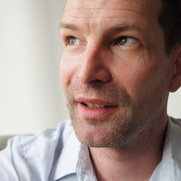
\includegraphics[width=0.3\textwidth]{images/Matthias_Schlossberger.png}
%	\caption{Matthias Schlo"sberger}
%	\label{fig:MS}
%\end{figure}


%\begin{figure}[h]
%	\centering
%	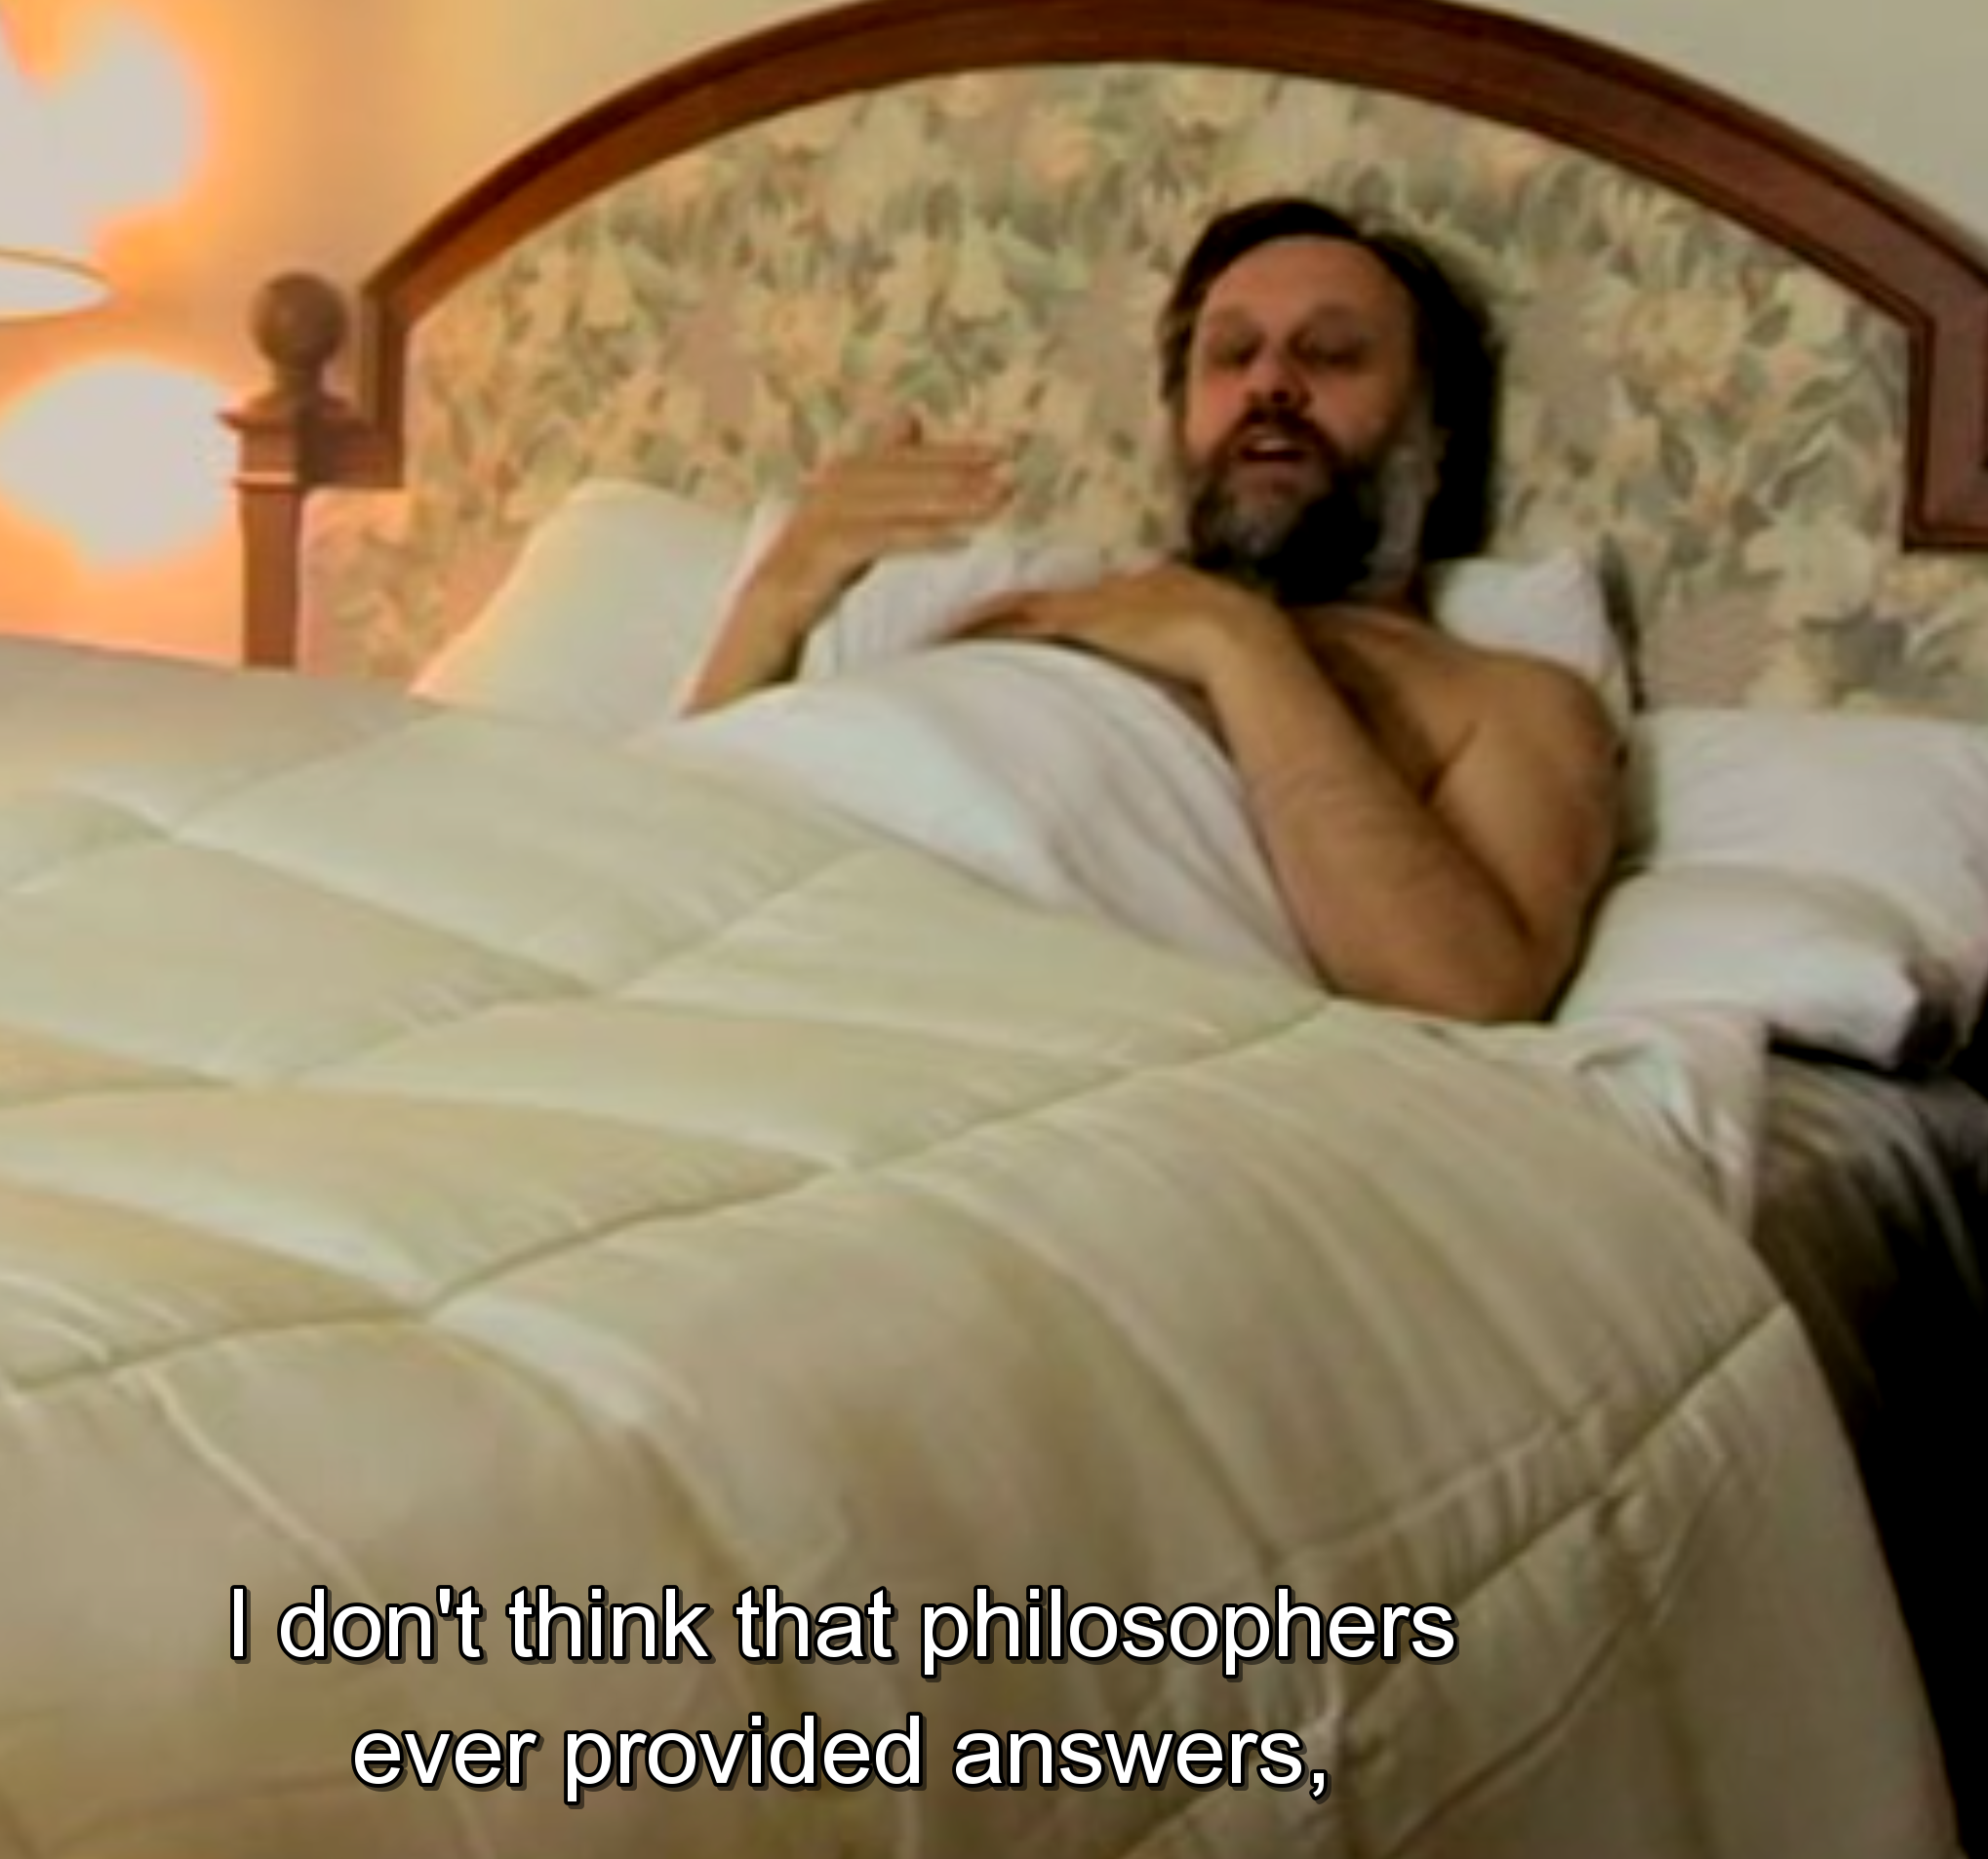
\includegraphics[width=0.5\textwidth]{images/template.png}
%	\caption{Template Bild}
%	\label{fig:template}
%\end{figure}

\end{document}
